% --------------------------------------------------------------------------- %
% Poster for the ECCS 2011 Conference about Elementary Dynamic Networks.      %
% --------------------------------------------------------------------------- %
% Created with Brian Amberg's LaTeX Poster Template. Please refer for the     %
% attached README.md file for the details how to compile with `pdflatex`.     %
% --------------------------------------------------------------------------- %
% $LastChangedDate:: 2011-09-11 10:57:12 +0200 (V, 11 szept. 2011)          $ %
% $LastChangedRevision:: 128                                                $ %
% $LastChangedBy:: rlegendi                                                 $ %
% $Id:: poster.tex 128 2011-09-11 08:57:12Z rlegendi                        $ %
% --------------------------------------------------------------------------- %
\documentclass[a0paper,portrait]{baposter}

\usepackage{relsize}		% For \smaller
\usepackage{url}			% For \url
\usepackage{epstopdf}	% Included EPS files automatically converted to PDF to include with pdflatex
\usepackage{cite}
\usepackage{xcolor}
\usepackage{caption}

\newcommand{\tabincell}[2]{\begin{tabular}{@{}#1@{}}#2\end{tabular}}
%%% Global Settings %%%%%%%%%%%%%%%%%%%%%%%%%%%%%%%%%%%%%%%%%%%%%%%%%%%%%%%%%%%

\graphicspath{{figures/}}	% Root directory of the pictures 
\tracingstats=2			% Enabled LaTeX logging with conditionals

%%% Color Definitions %%%%%%%%%%%%%%%%%%%%%%%%%%%%%%%%%%%%%%%%%%%%%%%%%%%%%%%%%

\definecolor{bordercol}{RGB}{40,40,40}
\definecolor{headercol1}{RGB}{186,215,230}
\definecolor{headercol2}{RGB}{80,80,80}
\definecolor{headerfontcol}{RGB}{0,0,0}
%\definecolor{boxcolor}{RGB}{186,215,230}
\definecolor{boxcolor}{RGB}{255,255,255}
%%%%%%%%%%%%%%%%%%%%%%%%%%%%%%%%%%%%%%%%%%%%%%%%%%%%%%%%%%%%%%%%%%%%%%%%%%%%%%%%
%%% Utility functions %%%%%%%%%%%%%%%%%%%%%%%%%%%%%%%%%%%%%%%%%%%%%%%%%%%%%%%%%%

%%% Save space in lists. Use this after the opening of the list %%%%%%%%%%%%%%%%
\newcommand{\compresslist}{
	\setlength{\itemsep}{1pt}
	\setlength{\parskip}{0pt}
	\setlength{\parsep}{0pt}
}

%%%%%%%%%%%%%%%%%%%%%%%%%%%%%%%%%%%%%%%%%%%%%%%%%%%%%%%%%%%%%%%%%%%%%%%%%%%%%%%
%%% Document Start %%%%%%%%%%%%%%%%%%%%%%%%%%%%%%%%%%%%%%%%%%%%%%%%%%%%%%%%%%%%
%%%%%%%%%%%%%%%%%%%%%%%%%%%%%%%%%%%%%%%%%%%%%%%%%%%%%%%%%%%%%%%%%%%%%%%%%%%%%%%

\begin{document}
\typeout{Poster rendering started}

%%% Setting Background Image %%%%%%%%%%%%%%%%%%%%%%%%%%%%%%%%%%%%%%%%%%%%%%%%%%
\background{
	\begin{tikzpicture}[remember picture,overlay]%
	\draw (current page.north west)+(-2em,2em) node[anchor=north west]
	{};
        %{\includegraphics[height=1.1\textheight]{background}};
	\end{tikzpicture}
}

%%% General Poster Settings %%%%%%%%%%%%%%%%%%%%%%%%%%%%%%%%%%%%%%%%%%%%%%%%%%%
%%%%%% Eye Catcher, Title, Authors and University Images %%%%%%%%%%%%%%%%%%%%%%
\begin{poster}{
	grid=false,
	%eyecatcher=false, 
	borderColor=bordercol,
	headerColorOne=headercol1,
	headerColorTwo=headercol2,
	headerFontColor=headerfontcol,
	boxColorOne=boxcolor,
	headershape=roundedright,
	headerfont=\Large\sf\bf,
	textborder=rectangle,
	background=user,
        %background=plain,
	headerborder=open,
        boxshade=plain,
        bgColorOne=white
}

%%% Eye Cacther %%%%%%%%%%%%%%%%%%%%%%%%%%%%%%%%%%%%%%%%%%%%%%%%%%%%%%%%%%%%%%%
%{
%	Eye Catcher, empty if option eyecatcher=false - unused
%}
%%% Title %%%%%%%%%%%%%%%%%%%%%%%%%%%%%%%%%%%%%%%%%%%%%%%%%%%%%%%%%%%%%%%%%%%%%
{\sf\bf QuickDough: A Rapid FPGA Accelerator Design Methodology Using Soft 
Coarse-Grained Reconfigurable Array Overlay
}
%%% Authors %%%%%%%%%%%%%%%%%%%%%%%%%%%%%%%%%%%%%%%%%%%%%%%%%%%%%%%%%%%%%%%%%%%
{
	\vspace{1em} Cheng Liu, Colin Yu Lin, Hayden Kwok-Hay So\\
	{\smaller liucheng@eee.hku.hk, linyu@eee.hku.hk, hso@eee.hku.hk}
}
%%% Logo %%%%%%%%%%%%%%%%%%%%%%%%%%%%%%%%%%%%%%%%%%%%%%%%%%%%%%%%%%%%%%%%%%%%%%
{
% The logos are compressed a bit into a simple box to make them smaller on the result
% (Wasn't able to find any bigger of them.)
\setlength\fboxsep{0pt}
\setlength\fboxrule{0pt}
  \fbox{
    \begin{minipage}{12em}
    \includegraphics[width=12em,height=12em]{hkulogo}
    \end{minipage}
  }
}

\headerbox{Background and Motivation}{name=motivation,column=0,row=0}{
The design productivity of developing an FPGA accelerator remains a major obstacle that hinders it from wide adoption. FPGA overlay which can be parametric HDL, pre-synthesized or pre-implemented circuit is a promising technique to tackle the design productivity challenge. It is beneficial to FPGA design productivity mainly from the following three aspects.
\begin{itemize}
\item It usually uses DFG or even high level language program as input, and thus raises the abstraction level of design entry.
\item It typically has coarser configuration granularity and simplifies the compilation. Therefore, it helps to reduce the compilation time.
\item It can be reused across the FPGA devices and parts, which indicates more convenient design reuse and portability.
\end{itemize}
}

\headerbox{SCGRA Based Accelerator}{name=scgra,column=0,below=motivation}{
Figure \ref{fig:scgra-acc} shows the structure of the soft coarse-grained reconfigurable array (SCGRA) based FPGA accelerator. As the implementation of the SCGRA has significant impact on the overall performance, one PE of the SCGRA is further presented in Figure \ref{fig:pe}.

\setlength\fboxsep{0pt}
\setlength\fboxrule{0pt}

\begin{center}
%\fcolorbox{white}{white!100}{
\fbox{
\begin{minipage}{19em}
\begin{center}
\includegraphics[width=0.9\linewidth]{scgra-accelerator}
\captionof{figure}{SCGRA Based FPGA Accelerator}
\label{fig:scgra-acc}
\end{center}
\end{minipage}
}
%}
\end{center}

\begin{center}
%\fcolorbox{white}{white!100}{
\fbox{
\begin{minipage}{19em}
\begin{center}
\includegraphics[width=0.9\linewidth]{pe}
\captionof{figure}{PE Structure}
\label{fig:pe}
\end{center}
\end{minipage}
}
%}
\end{center}

}

\headerbox{Conclusion}{name=conclusion, column=0,below=scgra,above=bottom}{
QuickDough using the SCGRA overlay as an intermediate compilation step simplifies the lengthy FPGA implementation. The time compiling from high level language program to CPU+FPGA system can be reduced by around two magnitudes. In addition, implementation with higher clock frequency resulting from the highly regular structure of SCGRA in combination with effective operation scheduling provides competitive performance compared to a commercial HLS based design. 
}

%\headerbox{References}{name=references,column=0,below=conclusion,above=bottom}{
%\smaller
%\vspace{-0.4em}
%\bibliographystyle{plain}
%\bibliography{refs}
%\bibliographystyle{plain}				
%\renewcommand{\section}[2]{\vskip 0.05em}
%\begin{thebibliography}{1}			
%\itemsep=-0.01em				
%\setlength{\baselineskip}{0.4em}
%\bibitem{ref1} Lavin, C. and Padilla, M. and Ghosh, S. and Nelson, B. and Hutchings, B. and Wirthlin, M., Using hard macros to reduce FPGA compilation time, International conference on Field Programmable Logic and Applications, 2010
%\bibitem{ref2} The LLVM compiler framework, http://llvm.org
%\bibitem{ref3} Cong, J. and Liu, B. and Neuendorffer, S. and Noguera, J. and Vissers, K. and Zhang, Z., High-level synthesis for FPGAs: From prototyping to deployment, IEEE Transactions on Computer-Aided Design of Integrated Circuits and Systems, 2011
%\end{thebibliography}
%} 

\headerbox{QuickDough}{name=quickdough,column=1,row=0}{
QuickDough an SCGRA based FPGA accelerator design methodology as shown in Figure \ref{fig:quickdough} is proposed to compile an application to a hybrid CPU+FPGA system. It can be roughly divivded into two parts: conventional software compilation and SCGRA customization and compilation. The SCGRA customization and compilation part is further detailed in Figure \ref{fig:scgra-compile}. 

\vspace{-0.2em}
\setlength\fboxsep{0pt}
\setlength\fboxrule{0pt}
\begin{center}
%\fcolorbox{white}{white!100}{
  \fbox{
    \begin{minipage}{19em}
      \begin{center}
        \includegraphics[width=0.92\linewidth]{framework}
        \captionof{figure}{QuickDough}
        \label{fig:quickdough}
      \end{center}
    \end{minipage}
}
\fbox{
    \begin{minipage}{19em}
      \begin{center}
        \includegraphics[width=0.68\linewidth]{scgra-compile}
        \captionof{figure}{SCGRA Customization and Compilation}
        \label{fig:scgra-compile}
      \end{center}
    \end{minipage}
}
%}
\end{center}

}

\headerbox{Experiment setup}{name=setup,column=1,span=2, above=bottom}{
We take four applications including matrix multiplication (MM), FIR filter, Kmean and Sobel edge detector as our benchmark. Each application is further provided with three different data sets as illustrated in Table \ref{tab:benchmark-config}. The benchmark was implemented on Zedboard using both QuickDough and Vivado HLS based design methodology. Since we haven't complete the SCGRA customization work, we just have two typical SCGRA configurations as an example. The configuration details are listed in Table \ref{tab:scgra-config}. 
\setlength\fboxsep{0pt}
\setlength\fboxrule{0pt}
\begin{center}
  \fbox{
    \begin{minipage}{40em}
      \begin{tabular}{c|c|c|c|c}
        \hline
        Benchmark & MM & FIR & Sobel & Kmean \\ \hline
        Parameters & Matrix Size & \tabincell{c}{\# of Input \\ \# of Taps+1} & \tabincell{c}{ \# of Vertical Pixels \\ \# of Horizontal Pixels} & \tabincell{c}{\# of Nodes \\ \# of Centroids \\ Dimension Size} \\ \hline
        Small & 10 & 40/50 & 8/8 & 20/4/2 \\ \hline
        Medium & 100 & 10000/50 & 128/128 & 5000/4/2  \\ \hline
        Large & 1000 & 100000/50 & 1024/1024 & 50000/4/2 \\ \hline
      \end{tabular}
      \captionof{table}{Detailed Configuration of The Benchmark}
      \label{tab:benchmark-config}
    \end{minipage}
  }

  \fbox{
    \begin{minipage}{40em}
      \begin{tabular}{c|c|c|c|c|c}
        \hline
            {Topology} & {SCGRA Size} & {Data Mem} & {Inst Mem} & {In/Out Buffer} & {Addr Buffer} \\ \hline
            {Torus} & {$2 \times 2$, $5 \times 5$} & $256 \times 32$bits & $1024 \times 72$bits & $2048 \times 32$bits & $4096 \times 32$bits \\ \hline
      \end{tabular}
      \captionof{table}{SCGRA Configuration}
      \label{tab:scgra-config}
    \end{minipage}
  }
\end{center}

}

\headerbox{Experiment}{name=experiment,column=2,row=0}{
Design productivity comparison is shown in Figure \ref{fig:hls-compilation-time} and \ref{fig:quickdough-compilation-time}. End-to-end performance is compared in Figure \ref{fig:real-perf}. Kernel simulation performance is compared in Figure \ref{fig:kernel-sim-perf}.

\begin{center}
  \includegraphics[width=0.99\linewidth]{HLS-Compilation-Time}
  \captionof{figure}{Compilation Time Using Vivado HLS Based Design Methodology}
  \label{fig:hls-compilation-time}
\end{center}

\begin{center}
  \includegraphics[width=0.99\linewidth]{QuickDough-Compilation-Time}
  \captionof{figure}{Compilation Time Using QuickDough}
  \label{fig:quickdough-compilation-time}
\end{center}

\begin{center}
  \includegraphics[width=0.99\linewidth]{real-perf}
  \captionof{figure}{Performance Normalized To Vivado-HLS 2K Buffer}
  \label{fig:real-perf}
\end{center}

\begin{center}
  \includegraphics[width=0.99\linewidth]{kernel-sim-perf}
  \captionof{figure}{Kernel Simulation Performance Normalized to Vivado-HLS 2K Buffer}
  \label{fig:kernel-sim-perf}
\end{center}


%\begin{center}
%  \includegraphics[width=0.99\linewidth]{impl-freq}
%  \captionof{figure}{Implementation Frequency}
%  \label{fig:impl-freq}
%\end{center}

}

\end{poster}
\end{document}
